\documentclass[11pt]{article}
\usepackage[margin=1in]{geometry}
\usepackage{lmodern}
\pdfinfoomitdate=1
\pdftrailerid{}
\pdfsuppressptexinfo=15
\usepackage{amsmath,amssymb,booktabs,graphicx,microtype}
\usepackage[round,authoryear]{natbib}
\usepackage[hidelinks]{hyperref}
\hypersetup{hidelinks,colorlinks=false,pdfborder={0 0 0}}
\newcommand{\result}[2]{#2}
\title{Employment at Fast-Food Restaurants around\newline New Jersey's 1992 Minimum-Wage Increase}
\author{Independent historical reconstruction}
\date{October 2026}
% [results-sha256:@@RESULTSHASH@@]
% [claim:C_SCOPE]
\begin{document}
\maketitle
\begin{abstract}
This paper reconstructs the short-run employment comparison around New Jersey's minimum-wage increase using public restaurant survey records and an independently written analysis. Among @B:primary.n@ restaurants with complete employment outcomes before and after the change, the New Jersey minus Pennsylvania contrast in changes is @B:primary.estimate@ full-time-equivalent employees per restaurant. The restaurant-level heteroskedasticity-robust standard error is @B:primary.std_error@. Alternative headcount definitions, chain exclusions, closure treatment, and interview-mode restrictions retain a positive point estimate. The contrast is driven by a small rise in New Jersey and a larger decline in Pennsylvania. It identifies a policy effect only under unverified parallel untreated trends and absence of anticipation, spillovers, and differential selection. There is one baseline survey and only two policy jurisdictions. Consequently, conventional restaurant-level intervals describe conditional sampling uncertainty and do not establish statewide causal significance. The exercise supports a bounded descriptive finding, not an unrestricted claim about minimum wages or a welfare recommendation. % [claim:C_MAIN] [claim:C_LIMIT]
\end{abstract}

\section{Introduction}
Minimum-wage changes provide a direct way to study firms' employment responses to a wage floor. A competitive labor-demand account predicts lower desired labor input when an increase is binding, holding product demand and productivity fixed. Recruitment frictions, turnover responses, market power, or price adjustment can alter that prediction. Establishing which channel dominates requires evidence beyond an observed employment contrast. This paper asks how employment changed at surveyed fast-food restaurants around New Jersey's increase, and states the additional assumptions needed for a causal answer. % [claim:C_SCOPE]

The institutional discontinuity is geographic and temporal. New Jersey legislation scheduled an hourly minimum of \$5.05 for April 1, 1992, following \$4.25 in the preceding year. The legislative history establishes that the increase had been enacted in advance; it was not an unanticipated randomized intervention \citep{nj1990}. Public-use survey records contain establishments in New Jersey and eastern Pennsylvania, employment and starting wages in a baseline wave, and a second observation late in the year. The comparison removes common time movements and permanent mean differences between the sampled groups, but does not remove differential state shocks. % [claim:C_POLICY] [claim:C_LIMIT]

The primary analysis uses @B:primary.n_nj@ New Jersey and @B:primary.n_pa@ Pennsylvania complete pairs. New Jersey employment rises by @B:nj.change@ FTE employees on average, while Pennsylvania employment changes by @B:pa.change@. Their difference is @B:primary.estimate@. This is a relative employment comparison: it does not mean that New Jersey restaurants each added that many workers, and it is not the change in the total number of restaurant jobs statewide. % [claim:C_DATA] [claim:C_MAIN]

The contribution is transparent verification of a historical question. All estimates are generated from acquired raw data using a short Python program; a separate base-R implementation checks the primary coefficient and variance calculations. The public archive's original analysis program and the original article are excluded. The accompanying record discloses model familiarity and accidental exposure to search snippets, including a reported coefficient and some supporting specification descriptions. The exercise therefore cannot claim uncontaminated discovery, although its numerical findings are independently computed. % [claim:C_SCOPE] [claim:C_REPRO]

The paper proceeds from the institutional setting and inferential literature to the sample, design, estimates, and sensitivity checks. An appendix derives the identification equation, equivalence of the change regression and the two-group contrast, and the variance formula step by step. The conclusion distinguishes a reproducible sample fact from a causal or policy conclusion. % [claim:C_SCOPE]

\section{Setting and Relation to the Literature}
The archived New Jersey law and committee statements document the scheduled wage-floor increase. Because the schedule was known before the baseline interviews, anticipation is a maintained concern rather than a feature eliminated by interviewing before the effective date. The first-wave instrument is headed January--March 1992, and the raw second-wave dates span November--December. The public records do not provide a restaurant-specific first-wave date. A causal interpretation would have to address adjustment between enactment, announcement, baseline interviewing, and the effective date. % [claim:C_POLICY] [claim:C_DATA] [claim:C_LIMIT]

The Pennsylvania establishments provide a contemporaneous comparison within the same restaurant chains. Their geographic proximity and common industry make shared shocks plausible, but neither implies identical untreated changes. The comparison is particularly vulnerable to a Pennsylvania-specific demand decline, differences in local labor markets, and cross-border substitution. The present records have neither a long baseline history nor sufficient local demand measures to distinguish those possibilities from a policy effect. % [claim:C_LIMIT]

The inferential question differs from counting restaurants. \citet{conley2005} emphasize that a small number of policy changes can make conventional difference-in-differences approximations inappropriate, and develop inference using a large set of nonchanging groups. This application lacks that large donor set. \citet{alvarez2023} study further inference issues with few treated units and heterogeneous timing. The latter paper motivates a boundary on interpretation rather than a new estimator here: a single common treatment date and two survey waves do not create the staggered-treatment comparisons addressed by many modern estimators. % [claim:C_INFERENCE]

These references are used to explain uncertainty, not to reconstruct anyone else's treatment estimate. The substantive literature search is deliberately limited by the benchmark's prohibition on reading the target article, target code, teaching replication answers, or published target results. The original survey producers are acknowledged through their public data archive. No novelty claim or comprehensive literature-coverage claim is made. % [claim:C_SCOPE] [claim:C_REPRO]

\section{Data and Measurement}
The source is the public archive offered on David Card's researcher webpage, with documentation attributing the New Jersey--Pennsylvania surveys to the original project. The acquisition script extracts only the raw ASCII file, codebook, readme, and survey instruments. The SAS program in the archive is excluded. SHA-256 hashes freeze each consumed file, the acquisition script, and the schema. Public download access is verified; no express redistribution license accompanies the source, so the package does not claim an open license for republishing the archive. The data-availability statement gives the access route. % [claim:C_DATA] [claim:C_REPRO] [data:D_RAW]

The raw file contains @B:audit.n_raw@ rows, comprising @B:nj.n_raw@ New Jersey and @B:pa.n_raw@ Pennsylvania establishments in Burger King, KFC, Roy Rogers, and Wendy's. A fixed-width parser uses the codebook's exact column positions and treats a dot as missing. The codebook labels the sheet number as unique, but two source rows share that identifier. They are preserved because they are distinct records; a generated source-row key prevents an unintended merge or deletion. The supplied sample is not treated as a probability sample of all restaurants. Entry of new restaurants and establishments outside the surveyed chains are not observed. % [claim:C_DATA]

The survey asks separately about full-time and part-time nonmanagement workers and managers or assistant managers. Define FTE headcount as full-time workers plus managers plus one-half of part-time workers. This is a headcount conversion, not observed paid hours. The calculation requires every included component to be observed; missing components are not replaced with zero. All @B:audit.permanent_closed@ permanently closed restaurants have post-wave employment components recorded as zero and remain in the primary calculation when baseline employment is observed. Temporary closure statuses do not automatically imply zero employment. % [claim:C_DATA]

Complete employment pairs are available for @B:primary.n@ establishments. The available-case baseline means and post-wave means use different samples: Pennsylvania has @B:pa.n_pre@ baseline and @B:pa.n_post@ post-wave employment observations, and New Jersey has @B:nj.n_pre@ and @B:nj.n_post@. Table~\ref{tab:means} instead reports a constant sample within each state. Selection into complete pairs is a limitation because missingness may depend on employment changes. The analysis reports observation counts explicitly for each outcome and variant. % [claim:C_DATA] [claim:C_LIMIT]

\begin{table}[htbp]\centering
\caption{Employment on a constant restaurant sample}\label{tab:means}
@@TABLE:means@@
\begin{minipage}{.95\linewidth}\small\medskip
Notes: FTE is full-time nonmanagers plus managers plus one-half of part-time nonmanagers. Means and changes are unweighted. Source rows refer to the complete downloaded file; pairs require all employment components in both waves. Permanent closures with recorded zero post employment are retained.
\end{minipage}
\end{table}

Starting wages refer to a nonmanagement entrant, not mean wages or the wage bill. Meal price is the sum of the reported soda, small fries, and entree prices, including tax; it is not a quantity-weighted price index. Opening hours are daily hours open. The full-time share includes managers in the numerator and all reported workers in the denominator. A closed establishment has no defined employment share and is omitted from that particular outcome. These distinctions matter when interpreting adjustment margins. % [claim:C_DATA] [claim:C_AUX]

\section{Estimand, Design, and Uncertainty}
Let $D_i$ indicate a New Jersey restaurant, and let $t=0,1$ denote the baseline and late-year observations. The primary observable target is
\begin{equation}
\delta_{\mathrm{obs}}=E[\Delta Y_i\mid D_i=1,R_i=1]
-E[\Delta Y_i\mid D_i=0,R_i=1],
\label{eq:did}
\end{equation}
where $R_i=1$ means complete employment components in both waves. It is a contrast on the retained sample. Under no relevant baseline anticipation, consistency, no spillovers to Pennsylvania, and equality of mean untreated changes for these sampled groups, the contrast equals an average effect for the observed treated group. Appendix~\ref{app:derivation} shows exactly where those assumptions enter. Conditioning on complete pairs introduces an additional selection requirement if treatment changes whether an outcome is observed. The estimand is not silently extended to all original establishments. % [claim:C_ESTIMAND] [claim:C_LIMIT]

The estimator is the coefficient on $D_i$ in
\begin{equation}
\Delta Y_i=\alpha+\delta D_i+u_i.
\label{eq:reg}
\end{equation}
OLS here equals the difference in mean changes. No weights, post-treatment controls, restaurant-level trend terms, or exposure-driven sample search are used. A supporting regression adds baseline chain indicators and company ownership. A second supporting specification uses the initial wage gap $G_i=D_i\max\{(5.05-w_i)/w_i,0\}$ in place of the state indicator. The gap coefficient is an association per unit of proportional exposure, not an instrumented elasticity: initial wages may reflect demand, productivity, or measurement error. % [claim:C_ESTIMAND] [claim:C_GAP]

With only one baseline wave, pre-policy trends cannot be estimated. A non-significant comparison of baseline levels would not test parallel trends; levels need not match under difference-in-differences. Similarly, unchanged starting wages in Pennsylvania would establish a wage comparison, not identical counterfactual employment trends. The design audit therefore marks parallel trends, anticipation, and spillovers inconclusive. It does not manufacture placebo dates or a pretrend test from unavailable observations. % [claim:C_LIMIT]

The table reports the conventional homoskedastic OLS standard error and the HC1 restaurant-level sandwich standard error. A stratified restaurant bootstrap resamples establishments separately within each state using a fixed seed. These procedures condition on the two observed state paths and assume appropriate restaurant independence. They do not represent random assignment of the policy and do not absorb a shared state-by-time shock. The number of policy jurisdictions is @B:audit.state_clusters@, so a many-state cluster asymptotic argument is unavailable. No statewide significance test is claimed. % [claim:C_INFERENCE]

A useful sensitivity interpretation is algebraic. If the mean untreated employment change in New Jersey would have exceeded that in Pennsylvania by $b$ FTE workers, then the policy effect consistent with the observed contrast is $\delta_{\mathrm{obs}}-b$. Thus a differential untreated change equal to the estimated contrast accounts for it entirely. The data do not identify $b$. This exposes the untestable comparison assumption without assigning a probability to it. % [claim:C_ESTIMAND] [claim:C_LIMIT]

\section{Employment Results}
Table~\ref{tab:main} reports a primary contrast of @B:primary.estimate@ FTE workers with HC1 standard error @B:primary.std_error@ and homoskedastic standard error @B:primary.se_homoskedastic@. The normal restaurant-level interval is [@B:primary.normal_low@, @B:primary.normal_high@], while the stratified bootstrap interval is [@B:primary.bootstrap_low@, @B:primary.bootstrap_high@]. These are conditional uncertainty summaries under restaurant independence. The observed pattern is inconsistent with a negative relative sample employment change, but uncertainty about the counterfactual state paths prevents treating that observation as an unconditional causal conclusion. % [claim:C_MAIN] [claim:C_INFERENCE]

\begin{table}[htbp]\centering
\caption{Employment-change regressions}\label{tab:main}
@@TABLE:main@@
\begin{minipage}{.95\linewidth}\small\medskip
Notes: Outcome is the change in FTE employment. Controls are baseline chain indicators and company ownership. The wage-gap specifications replace the state indicator with the proportional distance of the initial NJ wage below the new minimum; Pennsylvania exposure is zero. Gap coefficients are not directly comparable in units to state-indicator coefficients. Standard errors assume restaurant-level independence.
\end{minipage}
\end{table}

The controlled state coefficient is @B:controlled.estimate@, close to the raw contrast. Figure~\ref{fig:employment} shows why the relative comparison is positive: the New Jersey paired-sample mean changes modestly, while the Pennsylvania paired-sample mean declines. The available-case four-cell contrast is @B:crosssection.estimate@, close numerically to the paired estimate despite using changing samples. That proximity is a sample diagnostic, not evidence that missing outcomes are ignorable. % [claim:C_MAIN] [claim:C_ROBUST]

\begin{figure}[htbp]\centering
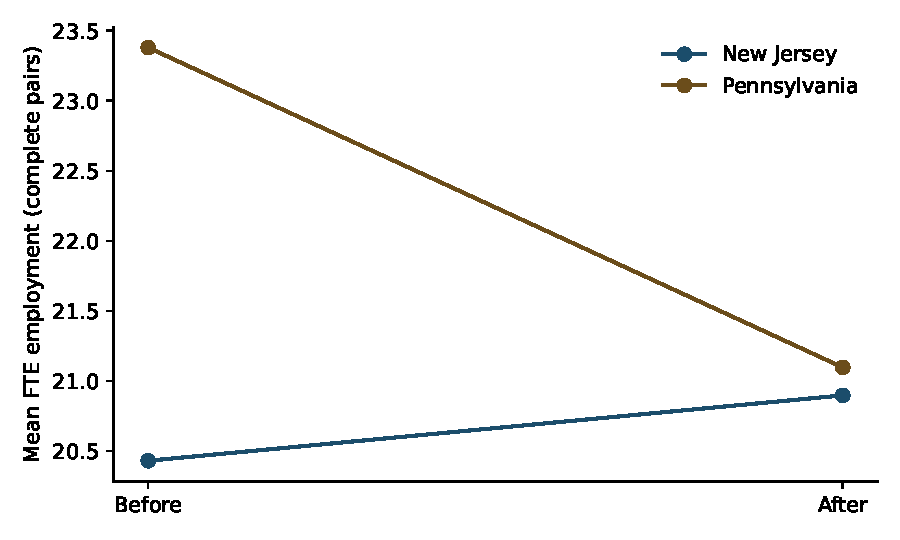
\includegraphics[width=.8\linewidth]{../../output/figures/employment.pdf}
\caption{Mean employment before and after the wage-floor change}\label{fig:employment}
\small Notes: Unweighted means for the same complete-pair restaurants used in the primary regression. Connecting two observations illustrates changes; it does not provide an event study or a test of trends.
\end{figure}

The estimated gap slope is @B:gap.estimate@, with @B:gap.n@ observations, and is @B:gap_controlled.estimate@ after chain and ownership controls. These positive associations are consistent with larger gains at more exposed restaurants, but they are not a separate source of exogenous assignment. In particular, noisy initial wages, wage-dependent establishment composition, or a recovery at initially low-wage locations can produce such a gradient. The paper does not identify a dose-response curve for arbitrary minimum-wage changes. % [claim:C_GAP]

\section{Sensitivity and Adjustment Margins}
Sensitivity checks address specific measurement and composition threats. Alternative part-time weights change the mapping from headcounts to labor input. Excluding managers changes both the outcome and the complete-component sample. Omitting permanent closures conditions on survival and therefore addresses a different population; it is not preferred because it can remove part of a policy response. Interview-mode and shore restrictions examine reporting and seasonal-composition differences. Leave-one-chain-out estimates test dependence on a chain's weight, and winsorization reduces the influence of extreme changes. Every variant is displayed without selecting on its standard error. % [claim:C_ROBUST]

\begin{table}[htbp]\centering
\caption{Sensitivity of the employment contrast}\label{tab:robust}
@@TABLE:robustness@@
\begin{minipage}{.95\linewidth}\small\medskip
Notes: Each row changes one rule from the primary contrast. All coefficients are NJ minus PA mean changes. Removing managers allows records missing manager counts to enter. Winsorization caps pooled changes at the first and ninety-ninth percentiles. Subset results change the target population and remain subject to the same comparison assumptions.
\end{minipage}
\end{table}

All displayed sensitivity coefficients remain positive. Their magnitudes are not identical: omitting Burger King yields @B:robust_omit_chain1.estimate@, while omitting KFC yields @B:robust_omit_chain2.estimate@. Consequently, a single common effect across chains is not established. The closure-excluding contrast is @B:robust_no_permanent.estimate@. Stability of these signs cannot refute a shared differential state shock or measurement error common to multiple variants. % [claim:C_ROBUST] [claim:C_LIMIT]

A diagnostic compares Pennsylvania restaurants with the @B:highwage.n_nj@ New Jersey complete-pair restaurants whose initial wage is at least the new minimum. The contrast is @B:highwage.estimate@ with HC1 standard error @B:highwage.std_error@. This differs in direction from the full sample and is imprecise. High-wage establishments are a selected group, not an untreated experiment: wage spillovers and differing trends remain possible. The diagnostic therefore cautions against interpreting one uniform state effect and does not validate or reject parallel trends by itself. % [claim:C_DIAGNOSTIC] [claim:C_LIMIT]

Table~\ref{tab:outcomes} shows a starting-wage change contrast of @B:outcome_starting_wage.estimate@ dollars per hour. Figure~\ref{fig:wages} displays the distributions, including the new wage floor. These wage observations provide evidence of changed reported entry pay. They do not measure hours paid, productivity, turnover, profits, or total payroll. The meal-price contrast is @B:outcome_meal_price.estimate@ dollars; opening hours and full-time share show different changes. These are auxiliary reduced-form descriptions on outcome-specific samples, and the paper does not claim to establish a pass-through, monopsony, or turnover mechanism. % [claim:C_AUX]

\begin{table}[htbp]\centering
\caption{Other reported restaurant outcomes}\label{tab:outcomes}
@@TABLE:outcomes@@
\begin{minipage}{.95\linewidth}\small\medskip
Notes: Outcome-specific complete pairs; all contrasts are unweighted changes. Meal price sums soda, small fries, and entree prices including tax. Full-time share includes managers and is undefined for zero total headcount. The reported standard errors condition on restaurant independence.
\end{minipage}
\end{table}

\begin{figure}[htbp]\centering
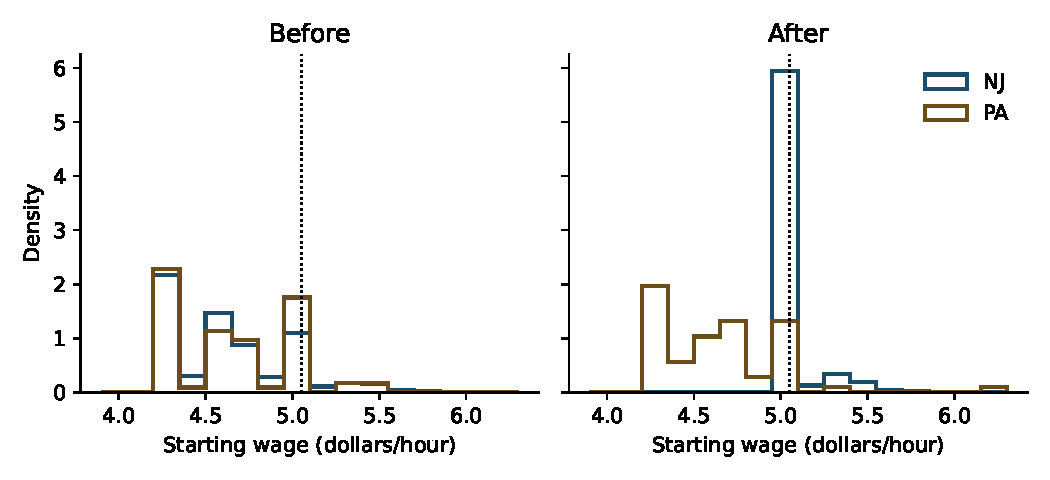
\includegraphics[width=.9\linewidth]{../../output/figures/wages.pdf}
\caption{Reported starting wages in the two survey waves}\label{fig:wages}
\small Notes: Histograms use all observed starting wages in each state and wave. The dotted line marks the new NJ floor. The displayed wage range does not impose a restriction on estimation samples.
\end{figure}

\section{Conclusion}
On the retained restaurant sample, employment rises slightly in New Jersey while falling in Pennsylvania, producing a positive relative change of @B:primary.estimate@ FTE employees per establishment. Independent parsing, explicit missing-value rules, raw-file checksums, and a second implementation make this sample finding reproducible. Alternative measurement and sample choices preserve its sign, while chain exclusions and high-wage comparisons reveal meaningful variation. % [claim:C_MAIN] [claim:C_ROBUST] [claim:C_REPRO]

The survey does not establish the counterfactual employment path. There is one baseline observation, advance notice of the policy, possible cross-border responses, outcome nonresponse, and only two policy jurisdictions. Those gaps remain after controls, robust restaurant-level standard errors, and bootstrap resampling. Under explicit parallel-trend, no-anticipation, no-spillover, and selection assumptions, the contrast can be interpreted as a short-run average effect for the observed treated restaurants. Without those assumptions it remains a descriptive relative employment change. No inference about national employment, long-run restaurant entry, welfare, or the desirability of a future wage floor is made. % [claim:C_LIMIT] [claim:C_ESTIMAND]

\appendix
\section{Identification and Estimator Derivations}\label{app:derivation}
The following derivations are algebraic consequences of stated assumptions. They are not formal kernel-checked proofs of an economic model, and they do not verify the assumptions from the data. Main-text equations~\eqref{eq:did} and~\eqref{eq:reg} rely on this appendix. % [claim:C_ESTIMAND]

\subsection{Potential-outcome decomposition}
Let $Y_{i1}(d)$ be post-wave employment under policy state $d\in\{0,1\}$ and $Y_{i0}(0)$ the baseline outcome without anticipation. For the observed treated sample assume $Y_{i0}=Y_{i0}(0)$ and $Y_{i1}=Y_{i1}(1)$. For the comparison sample assume $Y_{i0}=Y_{i0}(0)$ and $Y_{i1}=Y_{i1}(0)$, including the absence of spillovers. All expectations below condition on $R_i=1$; let $E_d[\cdot]=E[\cdot\mid D_i=d,R_i=1]$. % [claim:C_ESTIMAND]

Start with the observed contrast and substitute consistency:
\begin{align}
\delta_{\mathrm{obs}}
 &=E_1[Y_{i1}(1)-Y_{i0}(0)]
   -E_0[Y_{i1}(0)-Y_{i0}(0)].\label{eq:stepone}
\end{align}
Add and subtract $E_1[Y_{i1}(0)]$, which is permitted when the expectations are finite:
\begin{align}
\delta_{\mathrm{obs}}
 &=E_1[Y_{i1}(1)-Y_{i1}(0)]\notag\\
 &\quad+E_1[Y_{i1}(0)-Y_{i0}(0)]
       -E_0[Y_{i1}(0)-Y_{i0}(0)].\label{eq:steptwo}
\end{align}
Define $\tau_R=E_1[Y_{i1}(1)-Y_{i1}(0)]$ and $b_R$ as the difference of the final two expectations. Linearity of expectation therefore gives $\delta_{\mathrm{obs}}=\tau_R+b_R$. Parallel mean untreated changes means $b_R=0$, which implies $\delta_{\mathrm{obs}}=\tau_R$. If anticipation changes the baseline, the first substitution fails; if Pennsylvania responds to the policy, the comparison substitution fails. If $R_i$ depends on treatment, the conditioning populations may differ across potential states and $\tau_R$ cannot automatically be interpreted as an effect for a stable principal stratum. These are separate identifying requirements, not conclusions derived from the regression. % [claim:C_ESTIMAND] [claim:C_LIMIT]

\subsection{OLS and the difference in changes}
Write $z_i=\Delta Y_i$. OLS minimizes
\begin{equation}
Q(\alpha,\delta)=\sum_{D_i=0}(z_i-\alpha)^2
 +\sum_{D_i=1}(z_i-\alpha-\delta)^2.
\end{equation}
The derivative with respect to $\delta$ is $-2\sum_{D_i=1}(z_i-\alpha-\delta)$. Setting it to zero gives $\alpha+\delta=\bar z_1$, provided the treated sample is nonempty. The derivative with respect to $\alpha$ is minus twice the sum of both groups' residuals. The treated residual sum is already zero, so the control residual sum must also be zero, giving $\alpha=\bar z_0$ when the control sample is nonempty. Subtracting yields $\widehat\delta=\bar z_1-\bar z_0$. The design matrix has full rank because both treatment values occur. The objective is then strictly convex in the two fitted group means, ensuring this solution is the unique OLS minimizer. % [claim:C_ESTIMAND]

For a constant sample, $\bar z_d=\bar Y_{d1}-\bar Y_{d0}$ by linearity of finite sums with the same denominator. Substituting into the last identity produces the usual four-cell difference-in-differences expression. If baseline and post observations use different samples, this equality need not hold. That is why the main analysis fixes complete pairs and labels the available-case contrast separately. % [claim:C_ESTIMAND] [claim:C_DATA]

\subsection{Sampling variance and the omitted state shock}
Assume changes are independent within and across groups, have finite variances $\sigma_d^2$, and the group sizes $n_d$ are fixed. Variance of a mean is $\sigma_d^2/n_d$, because independent observations have zero pairwise covariance. Variance of the difference is therefore
\begin{equation}
\operatorname{Var}(\widehat\delta)=\frac{\sigma_1^2}{n_1}
 +\frac{\sigma_0^2}{n_0}.
\end{equation}
Replacing each population variance by its within-group sample variance gives the separate-group standard error reported in the results file. The HC1 matrix estimator is
\begin{equation}
\widehat V_{\mathrm{HC1}}
=\frac{n}{n-k}(X'X)^{-1}
 \left(\sum_i x_i x_i'\widehat u_i^2\right)(X'X)^{-1},
\end{equation}
with $k$ fitted coefficients. Its state-coefficient element uses the OLS residuals and applies a degrees-of-freedom multiplier. The homoskedastic estimator instead replaces the central matrix by $(X'X)\widehat\sigma^2$, with $\widehat\sigma^2=\sum_i\widehat u_i^2/(n-k)$, resulting in $\widehat\sigma^2(X'X)^{-1}$. These formulas are implemented directly and independently verified in base R. % [claim:C_INFERENCE] [claim:C_REPRO]

Now let $z_i=\mu_d+a_d+e_i$, where $a_d$ is a common state change shock and $e_i$ is an independent restaurant disturbance. Averaging gives $\bar z_d=\mu_d+a_d+\bar e_d$. Subtracting yields $\widehat\delta=(\mu_1-\mu_0)+(a_1-a_0)+(\bar e_1-\bar e_0)$. Increasing restaurant counts reduces the variance of the last term but leaves $a_1-a_0$ intact. Restaurant resampling holds both common shocks fixed, so it cannot estimate the uncertainty that those shocks create. With only two observed jurisdictions, the present design does not consistently learn their distribution. % [claim:C_INFERENCE] [claim:C_LIMIT]

\section{Replication and Audit Record}
Run \texttt{python3 scripts/run\_all.py} from the attempt directory. The master verifies the frozen raw checksums, recomputes the processed data, regressions, bootstrap, tables and figures, regenerates this manuscript from its source template, then invokes the unchanged research harness. The master reports actual return codes; failure of a delivery gate does not delete or suppress computed results. Dependencies and the seed are recorded in the environment file. All analysis paths are relative to the attempt directory. % [claim:C_REPRO]

The code-to-exhibit mapping is direct: \path{scripts/analyze.py} generates the employment means, regression table, sensitivity table, auxiliary-outcome table, and both figures. The manuscript builder, \path{scripts/build_package.py}, inserts those generated tables and binds displayed numbers to \path{research/results.json}. Data construction uses fixed-width fields and explicit complete-component rules. The code's primary coefficient equals a separately calculated difference of group means to numerical tolerance. The base-R check reproduces the coefficient and both reported analytical standard errors. % [claim:C_REPRO]

The design gate remains nonpassing where the data cannot resolve anticipation, parallel trends, spillovers, and policy-level inference. Bibliographic discovery is constrained and does not reproduce the target article's argument or every original table. Search-result numeric exposure and model familiarity are retained in \texttt{research/contamination.json}; nothing in the pipeline can erase that exposure. The manuscript is a bounded reconstruction with disclosed limitations, not evidence of an uncontaminated historical discovery or journal acceptance. % [claim:C_SCOPE] [claim:C_LIMIT] [claim:C_REPRO]

\subsection*{Data availability}
The original producer's public dataset page is \url{https://davidcard.berkeley.edu/data_sets.html}, which links the archived \texttt{njmin.zip}. The replication acquisition script downloads that archive and reads only the eligible raw data and documentation. A checksum manifest identifies the exact retrieved bytes. No confidential addresses or telephone numbers are available in the consumed public file, and no private data are used. Reusers should verify applicable redistribution permissions; this local analysis does not supply a new license. % [claim:C_DATA] [claim:C_REPRO]

\begin{thebibliography}{9}
\bibitem[Alvarez and Ferman(2023)]{alvarez2023}
Alvarez, Luis, and Bruno Ferman. 2023.
``Extensions for Inference in Difference-in-Differences with Few Treated Clusters.''
arXiv:2302.03131. \url{https://arxiv.org/abs/2302.03131}.
\bibitem[Conley and Taber(2005)]{conley2005}
Conley, Timothy, and Christopher Taber. 2005.
``Inference with Difference in Differences with a Small Number of Policy Changes.''
NBER Technical Working Paper 312. \url{https://doi.org/10.3386/t0312}.
\bibitem[New Jersey State Library(1990)]{nj1990}
New Jersey State Library. 1990.
``Minimum Wage---Increase to \$5.05 by 1992.''
Legislative History, Laws of 1990, Chapter 18, Assembly Bill 13.
\url{https://repo.njstatelib.org/items/af2bca87-0109-4742-8836-2684cd6e2fcf}.
% [claim:C_SCOPE] [claim:C_POLICY] [claim:C_INFERENCE]
\end{thebibliography}
\end{document}
